%%%%%%%%%%%%%%%%%%%%%%%%%%%%%%%%%%%%%%%%%
% Fancyslides Presentation
% LaTeX Template
% Version 1.0 (30/6/13)
%
% This template has been downloaded from:
% http://www.LaTeXTemplates.com
%
% The Fancyslides class was created by:
% Paweł Łupkowski (pawel.lupkowski@gmail.com)
%
% License:
% CC BY-NC-SA 3.0 (http://creativecommons.org/licenses/by-nc-sa/3.0/)
%
%%%%%%%%%%%%%%%%%%%%%%%%%%%%%%%%%%%%%%%%%

%----------------------------------------------------------------------------------------
%	PACKAGES AND OTHER DOCUMENT CONFIGURATIONS
%----------------------------------------------------------------------------------------

\documentclass{fancyslides}

\usepackage[utf8]{inputenc} % Allows the usage of non-english characters
\usepackage{pgfplots}
\usepackage{tikz}							%% Uncomment if you're using diagrams
\usetikzlibrary{calc}
\usepackage{times} % Use the Times font
\usepackage{booktabs} % Allows the use of \toprule, \midrule and \bottomrule in tables
%\usepackage{biblatex}

\graphicspath{{Images/}{../Images}} % Location of the slide background and figure files


% Beamer options - do not change
\usetheme{default} 
\setbeamertemplate{navigation symbols}{} % Disable the slide navigation buttons on the bottom of each slide
\setbeamercolor{structure}{fg=\yourowntexcol} % Define the color of titles and fixed text elements (e.g. bullet points)
\setbeamercolor{normal text}{fg=\yourowntexcol} % Define the color of text in the presentation

% Page count on bottom of page
\addtobeamertemplate{navigation symbols}{}{%
    \usebeamerfont{footline}%
    \usebeamercolor[fg]{footline}%
    \hspace{1em}%
    \insertframenumber/\inserttotalframenumber
}
\setbeamercolor{footline}{fg=blue}
%------------------------------------------------
% COLORS
% The following colors are predefined in this class: white, black, gray, blue, green and orange

% Define your own color as follows:
%\definecolor{pink}{rgb}{156,0,151}

\newcommand{\structureopacity}{0.75} % Opacity (transparency) for the structure elements (boxes and circles)

\newcommand{\strcolor}{blue} % Set the color of structure elements (boxes and circles)
\newcommand{\yourowntexcol}{white} % Set the text color

\newcommand\gauss[2]{1/(#2*sqrt(2*pi))*exp(-((x-#1)^2)/(2*#2^2))}

%------------------------------------------------
% TIKZ SETTINGS
\tikzset{
  invisible/.style={opacity=0},
  visible on/.style={alt={#1{}{invisible}}},
  alt/.code args={<#1>#2#3}{%
    \alt<#1>{\pgfkeysalso{#2}}{\pgfkeysalso{#3}} % \pgfkeysalso doesn't change the path
  },
}

%----------------------------------------------------------------------------------------
%	TITLE SLIDE
%----------------------------------------------------------------------------------------

\newcommand{\titlephrase}{Introduction to Gaussian Processes} % Presentation title
\newcommand{\name}{Matthew Lee} % Presenter's name
\newcommand{\affil}{Imperial College London} % Presenter's institution
\newcommand{\email}{matthew.lee13@imperial.ac.uk} % Presenter's email address

\begin{document}

\startingslide % This command inserts the title slide as the first slide

%----------------------------------------------------------------------------------------
%	PRESENTATION SLIDES
%----------------------------------------------------------------------------------------
%----------------------------------------------------------------------------------------
%	INTRODUCTION
%----------------------------------------------------------------------------------------
\logo{\includegraphics[scale=.2]{Biomedia_main.pdf}}
\usebackgroundtemplate{\includegraphics[height=\paperheight]{graph_paper.jpg}} % Slide background image
%------------------------------------------------
\begin{frame}
	\pointedsl{Aims}
\end{frame}
%------------------------------------------------
\begin{frame}
	\itemized{
		\large
		\item Constructing a GP
		\item A simple example
		\item Why is this useful?
	}
\end{frame}
%------------------------------------------------
\begin{frame}
	\misc{
		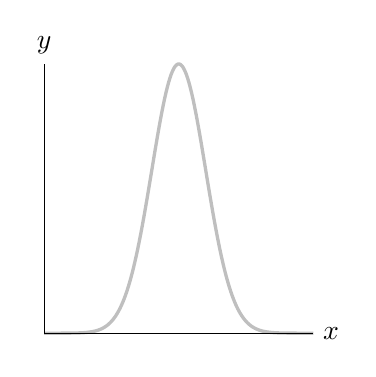
\begin{tikzpicture}
			\put(0,0){
				\begin{axis}[
					no markers, domain=0:10, samples=200,
					axis lines*=left, xlabel=$x$, ylabel=$y$,
					every axis y label/.style={at=(current axis.above origin),anchor=south},
					every axis x label/.style={at=(current axis.right of origin),anchor=west},
					height=5cm, width=5cm,
					xtick=\empty, ytick=\empty,
					enlargelimits=false, clip=false, axis on top,
					grid = major,
				]
				\addplot[gray!50, very thick, -] {\gauss{5}{1}};
				\end{axis}
			}
		\end{tikzpicture}
		
		$f(x \; | \; \mu, \sigma) = \frac{1}{\sigma\sqrt{2\pi} } \; e^{ -\frac{(x-\mu)^2}{2\sigma^2} }$

	}
\end{frame}
%------------------------------------------------
\begin{frame}
	\misc{
		\[
f_{\mathbf x}(x_1,\ldots,x_k) =
\frac{1}{\sqrt{(2\pi)^{k}|\boldsymbol\Sigma|}}
\exp\left(-\frac{1}{2}({\mathbf x}-{\boldsymbol\mu})^\mathrm{T}{\boldsymbol\Sigma}^{-1}({\mathbf x}-{\boldsymbol\mu})
\right)
		\]
	}
\end{frame}
%------------------------------------------------
\begin{frame}
	\misc{
		\[
\lim_{k\to \infty} \left(f_{\mathbf x}(x_1,\ldots,x_k) =
\frac{1}{\sqrt{(2\pi)^{k}|\boldsymbol\Sigma|}}
\exp\left(-\frac{1}{2}({\mathbf x}-{\boldsymbol\mu})^\mathrm{T}{\boldsymbol\Sigma}^{-1}({\mathbf x}-{\boldsymbol\mu})
\right)\right)
		\]
	}
\end{frame}
%------------------------------------------------

\begin{frame}
	\pointedsl{Questions?}
\end{frame}
%----------------------------------------------------------------------------------------
%	NOTES
%----------------------------------------------------------------------------------------
%The Eyescream Project: Uses generative models to compete with discriminative models


%----------------------------------------------------------------------------------------


\end{document}